\section{Results}\label{sec:results}

In order to evaluate the precision navigation system developed in this thesis, a number of different experiments, both on HARLIE and in simulation, were conducted. There were three major sets of experiments conducted: repeatability tests of the entire precision navigation system, tests to evaluate the acceptable initial conditions for phase space steering and tests to validate the splicing method used.

\subsection{Path Following Precision}\label{subsec:path_following_precision}

\begin{figure}
\centering
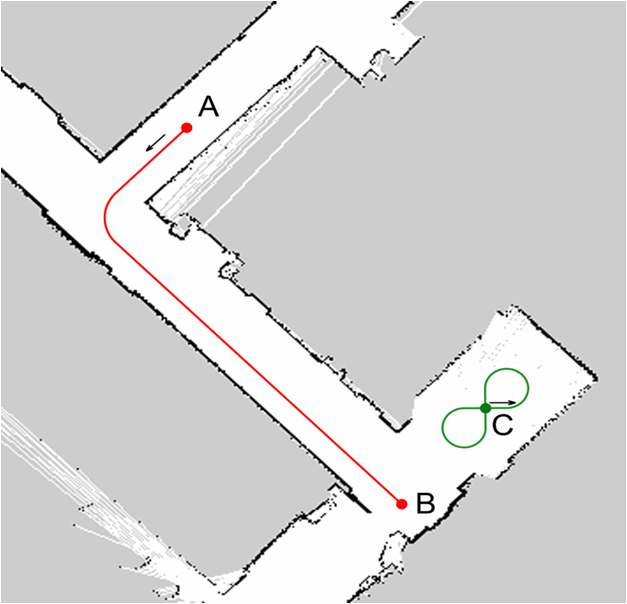
\includegraphics[width=0.75\textwidth]{images/path_following_paths}
\caption{Paths for Navigation Precision Tests \label{fig:path_following_paths}}
\end{figure}

The first set of tests run to evaluate the performance of the precision navigation system described in this thesis were designed to measure the actual precision with which it executed a path. To do this, two distinct sample paths were created on the second floor of the Case Western Reserve University Glennan building; these paths are shown overlaid to scale on the \emph{a priori} map in \autoref{fig:path_following_paths}. The first path, called the ``L'' path, is in red, which proceeds down a hallway from point A to point B. The second path, called the ``figure-8'' path, is in green. In the figure-8, the robot starts at point C facing in the direction indicated by the arrow and then proceeds around each arc before stopping again at point C. Throughout this section, a “run” on the L path refers to one complete trip starting at point A and ending at point B. For the figure-8 path, a “run” is defined as starting at point C, going through both the top and bottom loops and stopping again at point C. For the precision navigation system, both of these paths were described geometrically as a sequence of arcs and line segments.

To generate the path following performance measurements, five independent runs of the experiment were gathered while logging the pose of the robot with respect to the fixed origin of the \emph{a priori} map as estimated by the localization subsystem described in \autoref{sec:localization}. After all five runs were completed, the logged data was post-processed to compute lateral offsets relative to the desired path at each of the logged poses. The root-mean-square (RMS) of those lateral offsets was calculated for each individual run. This RMS value was averaged over all five runs of a given experiment and the standard deviation of those RMS values was calculated to generate a measure of repeatability.

\begin{figure}
\centering
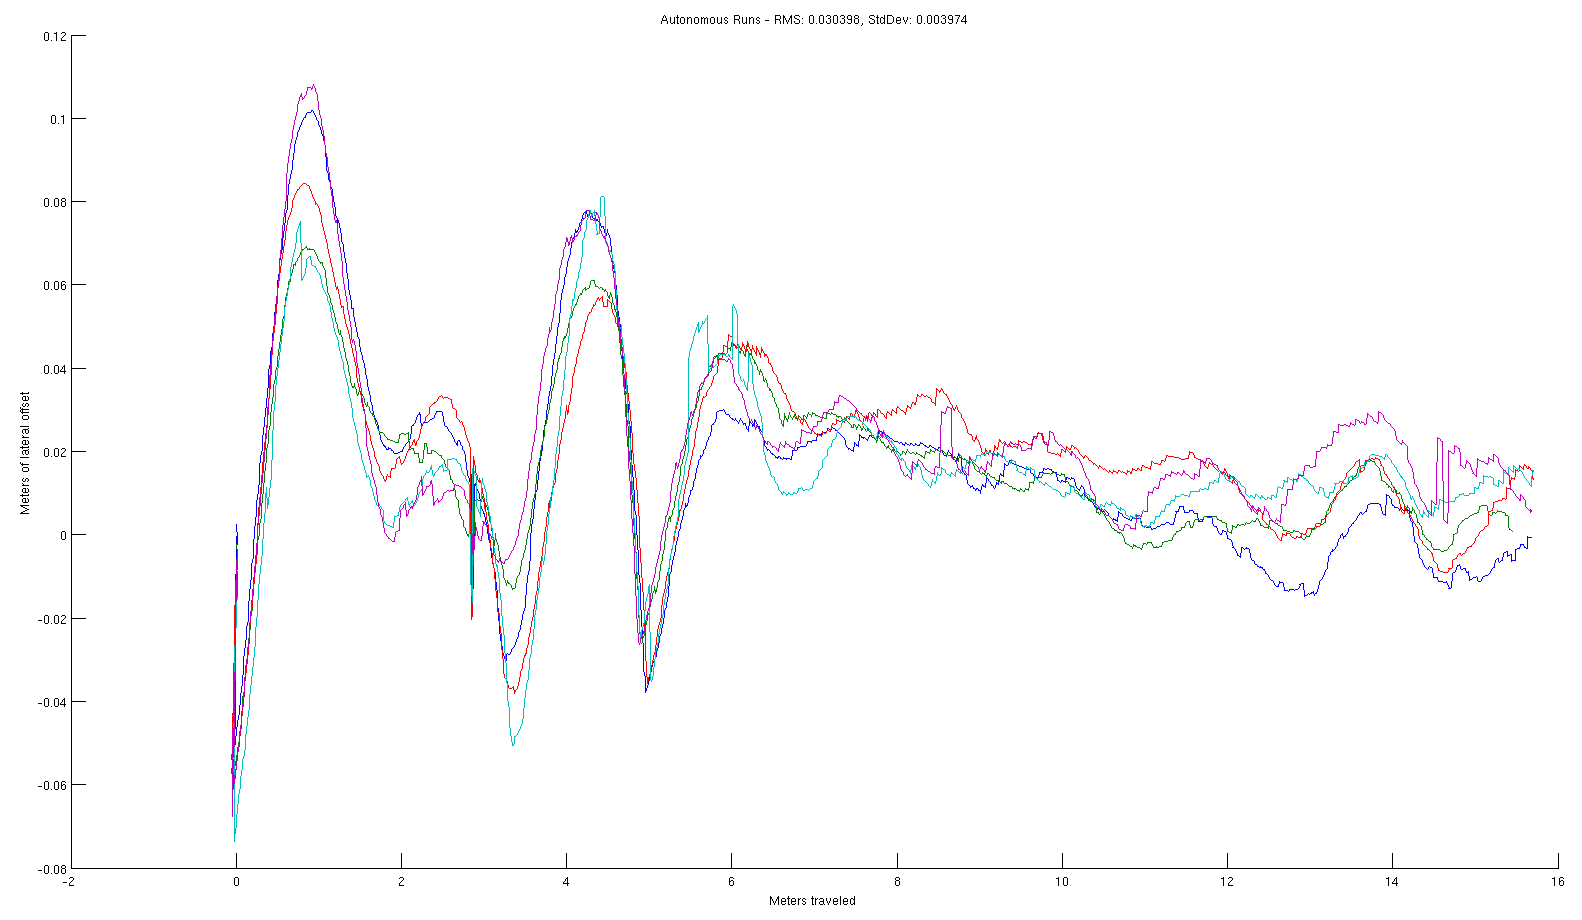
\includegraphics[width=0.95\textwidth]{images/l_path_autonomous_error}
\caption[Precision Navigation Error on the L Path]{Precision Navigation Error on the L Path. The X-axis is meters traveled and the Y-axis is meters of lateral offset}
\label{fig:l_path_autonomous_error}
\end{figure}

Performance was measured in terms of RMS lateral offsets from the defined path. \autoref{fig:l_path_autonomous_error} shows the performance of autonomous runs of the precision navigation system on the L path. As can be seen, the path following errors were small and highly repeatable. Lateral errors were just over three centimeters RMS, and this result was repeatable with a standard deviation of less than four millimeters.

\begin{figure}
\centering
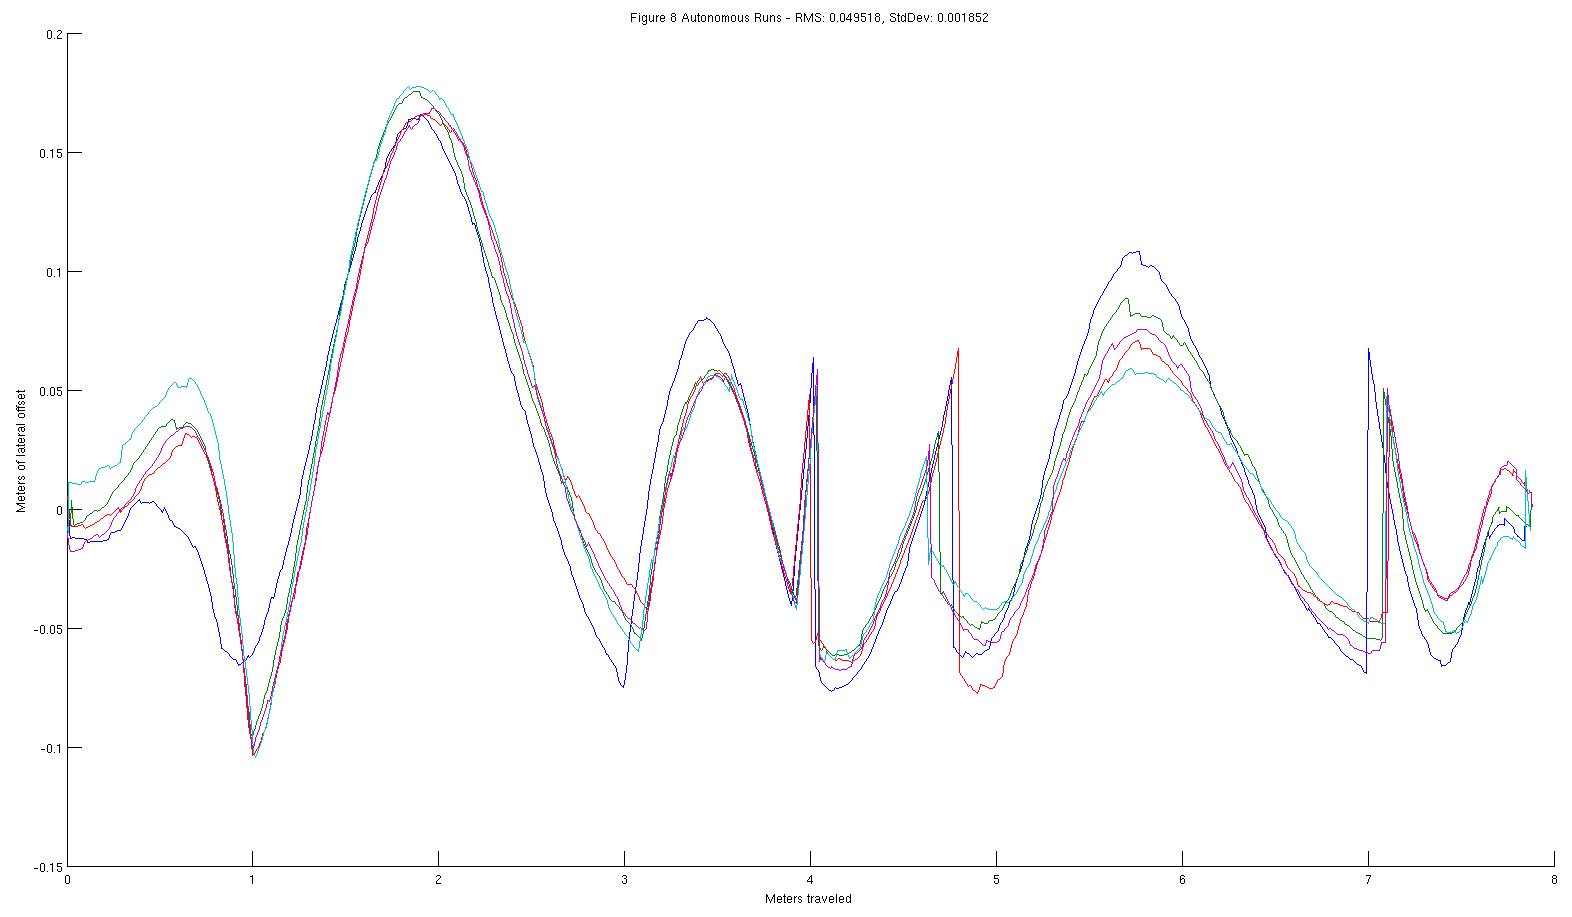
\includegraphics[width=0.95\textwidth]{images/fig_8_autonomous_error}
\caption[Precision Navigation Error on the Figure 8 Path]{Precision Navigation Error on the Figure 8 Path. The X-axis is meters traveled and the Y-axis is meters of lateral offset}
\label{fig:fig_8_autonomous_error}
\end{figure}

The figure-8 test path had relatively tight turn radii (2ft), making it a more challenging path. Again, performance was measured in terms of RMS lateral offsets from the defined path. \autoref{fig:fig_8_autonomous_error} shows the performance of autonomous runs of the precision navigation system on the figure-8 path. As can be seen, the path following errors were small and highly repeatable. Lateral errors were less than five centimeters RMS, and this result was repeatable with a standard deviation of less than two centimeters.

The results for both of these tests show that the precision navigation described in this thesis is sufficiently precise for the use cases previously described, such as navigating a robotic wheelchair through an ADA-compliant doorway that would have under seven centimeters of clearance on either side of the robot. The majority of the lateral offset error shown in \autoref{fig:l_path_autonomous_error} and \autoref{fig:fig_8_autonomous_error} occurs at changes in the path curvatures. For example, in the L path error graph, the large variations in lateral offset at approximately one and four meters of distance traveled coincide with entering and leaving the arc between hallways. After leaving the arc (after approximately six meters traveled), the lateral offset error becomes much less variable as the robot reaches the long, straight section of the L path.

\subsection{Phase Space Steering Initial Condition Tests}\label{subsec:phase_space_steering_skills}

Another set of tests was conducted to gather information about the attraction region of the phase space steering algorithm (see \autoref{subsubsec:phase_space_steering}) as well as gather quantitative data on the acceptable initial conditions for the path planner (see \autoref{sec:path_planning}). Two different tests were conducted: the ``door'' test (see \autoref{subsubsec:door_test}) and the ``tangent'' test (see \autoref{subsubsec:tangent_test}). Note that all of the results of these tests depend on the gains and other parameters, as well as steering algorithm, used. For these tests, phase space steering was selected as the steering algorithm, with the following gains and parameters (as described in \autoref{subsubsec:phase_space_steering}: $k_v = 0.1$, $k_\Psi = 1.0$ and the slope of the phase space mapping function $s = -1.0$.

\subsubsection{``Door'' Test}\label{subsubsec:door_test}

The ``door'' test is designed to ask: Given a set of initial conditions (lateral offset and heading error), will phase space steering converge onto the path before reaching the door? This test involved commanding a path composed of a single straight line segment, positioned and oriented such that the line passes through the center of a doorway, while positioning the robot such that it had different lateral offsets and heading offsets to the path. These tests were conducted both in the Gazebo simulation environment described in \autoref{subsec:simulation_setup} and a subset of those results were tested on HARLIE to verify that the simulation results transfered to the physical robot. Simulation results are shown in \autoref{fig:door_skill_sim_results}.

\begin{figure}
\centering
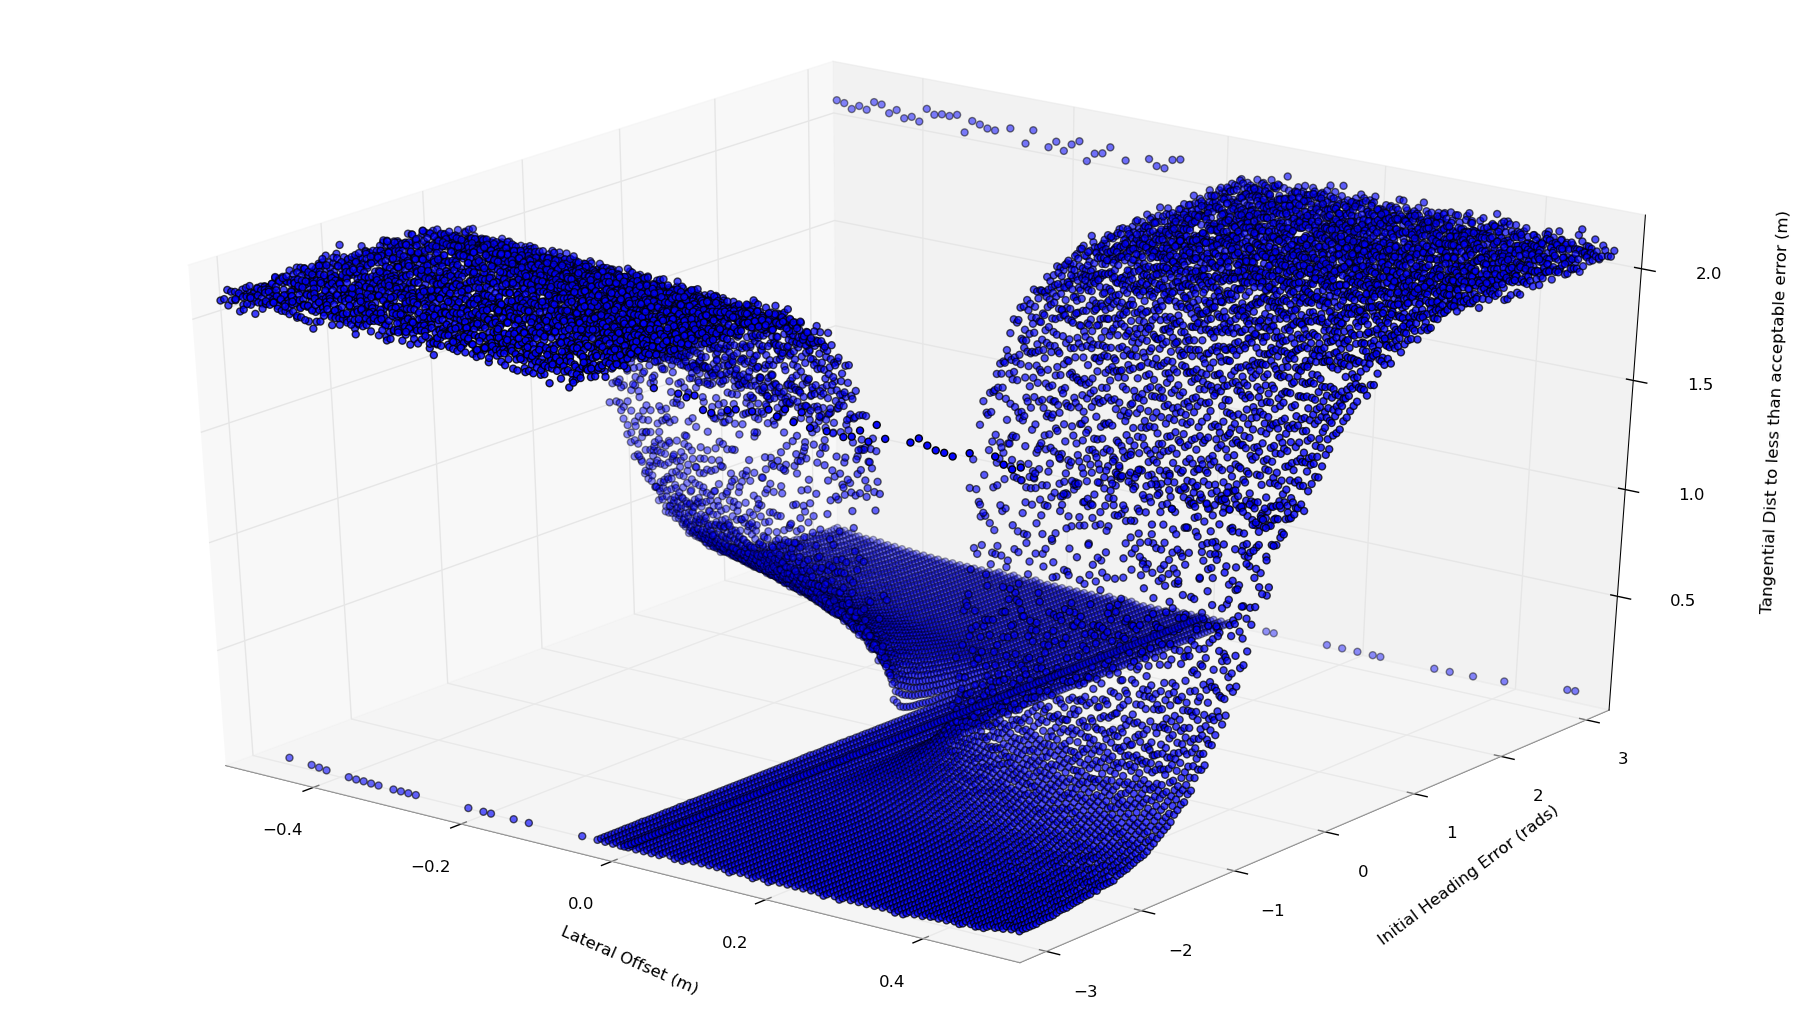
\includegraphics[width=0.95\textwidth]{images/acceptable_error_surface}
\caption[``Door'' Test Simulation Results]{``Door'' Test Simulation Results. The X-axis is the Initial Heading Error (rads), the Y-axis is the Initial Lateral Offset Error (m) and the Z-axis is the Tangential Distance to Path Convergence (m)}
\label{fig:door_skill_sim_results}
\end{figure}

There are a number of useful results shown in \autoref{fig:door_skill_sim_results}. The first is that the performance of the phase space steering algorithm is symmetric about the XZ-plane. This makes sense for HARLIE, as a negative heading error and positive lateral offset will have the robot already facing towards the path and a positive heading error and negative lateral offset will also have the robot facing towards the path. Any situation where the robot's initial conditions have it facing the path is much easier for the steering algorithm to converge onto the path in less distance along the path than a situation where the robot's initial conditions have it facing away from the path.

A second result from the simulation experiments is the actual shape of the experimental data. This shape implies that the way to converge to the path with the least distance traveled along the path is to face the path as quickly as possible before beginning to move fowards. Logically, this makes sense -- moving forwards directly towards the path will converge more quickly than moving forwards at an angle towards the path. Essentially, the way to converge to the path with the least tangential distance traveled is to follow the gradient of this surface at whichever lateral offset and heading error the algorithm has -- which is exactly what the phase space steering algorithm is designed to do.

This experiment also yielded information as to the minimum tangential distance required to converge to the path, given a set of initial conditions. This data can be used to determine whether, given a set of initial conditions and a doorway that must be traversed, a path planner must replan from the initial conditions to the path or if no replanning is required because there is enough distance before the door to converge to the path before reaching the door. For example, the data collected in simulation implies that, given a lateral offset of twenty-five centimeters and an initial heading error of fourty-five degrees, the robot must be at least thirty-one centimeters away perpendicularly from the doorway in order to safely pass through the doorway. A number of runs were conducted with HARLIE to validate these results; these tests with the physical system confirmed the simulation results. See \autoref{fig:door_skill_harlie_results} for some examples of HARLIE while conducting these tests.  There are two different initial conditions shown (see \autoref{fig:door_skill_harlie_results_initial_a} and \autoref{fig:door_skill_harlie_results_initial_b}), as well as HARLIE clearing the doorway (see \autoref{fig:door_skill_harlie_results_clearing_doorway}).

\begin{figure}
\centering
\subfloat[Initial Condition A]{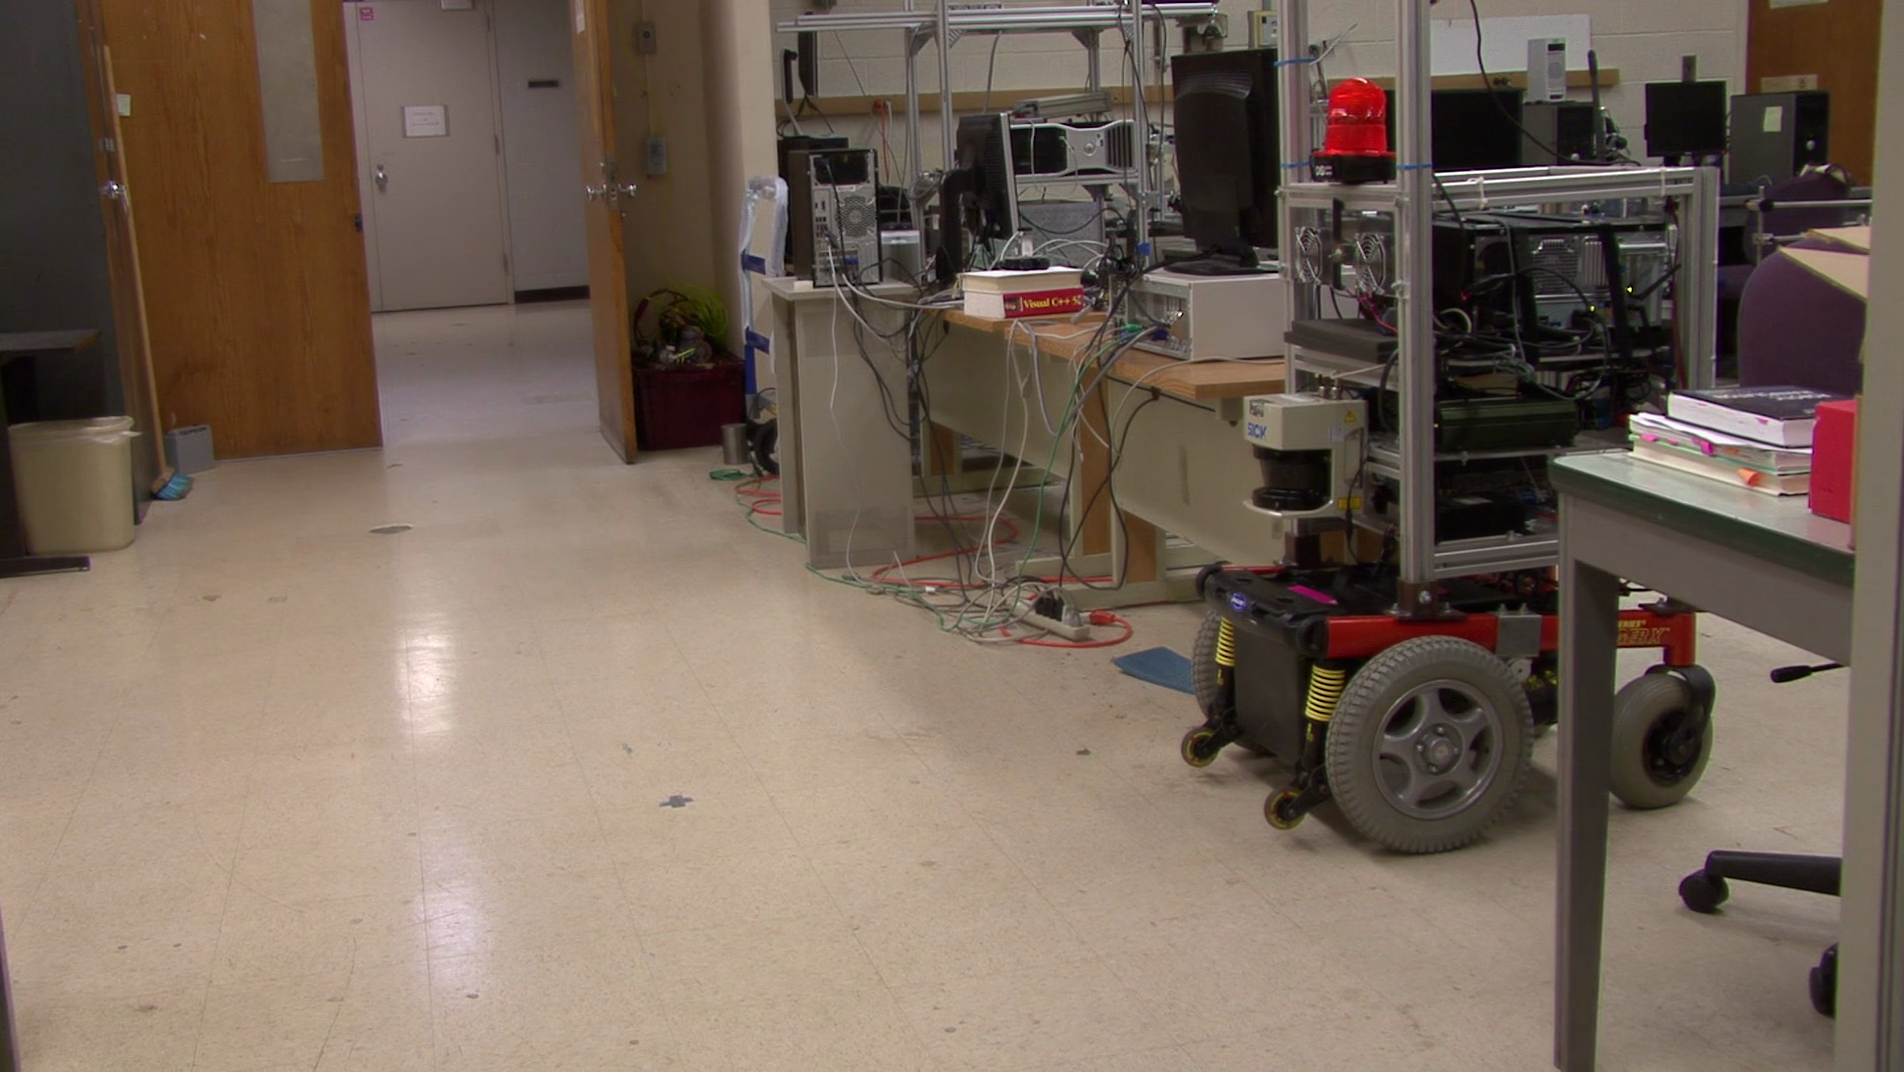
\includegraphics[width=0.49\textwidth]{images/door_skill_harlie_initial_a}\label{fig:door_skill_harlie_results_initial_a}}
\hfill
\subfloat[Initial Condition B]{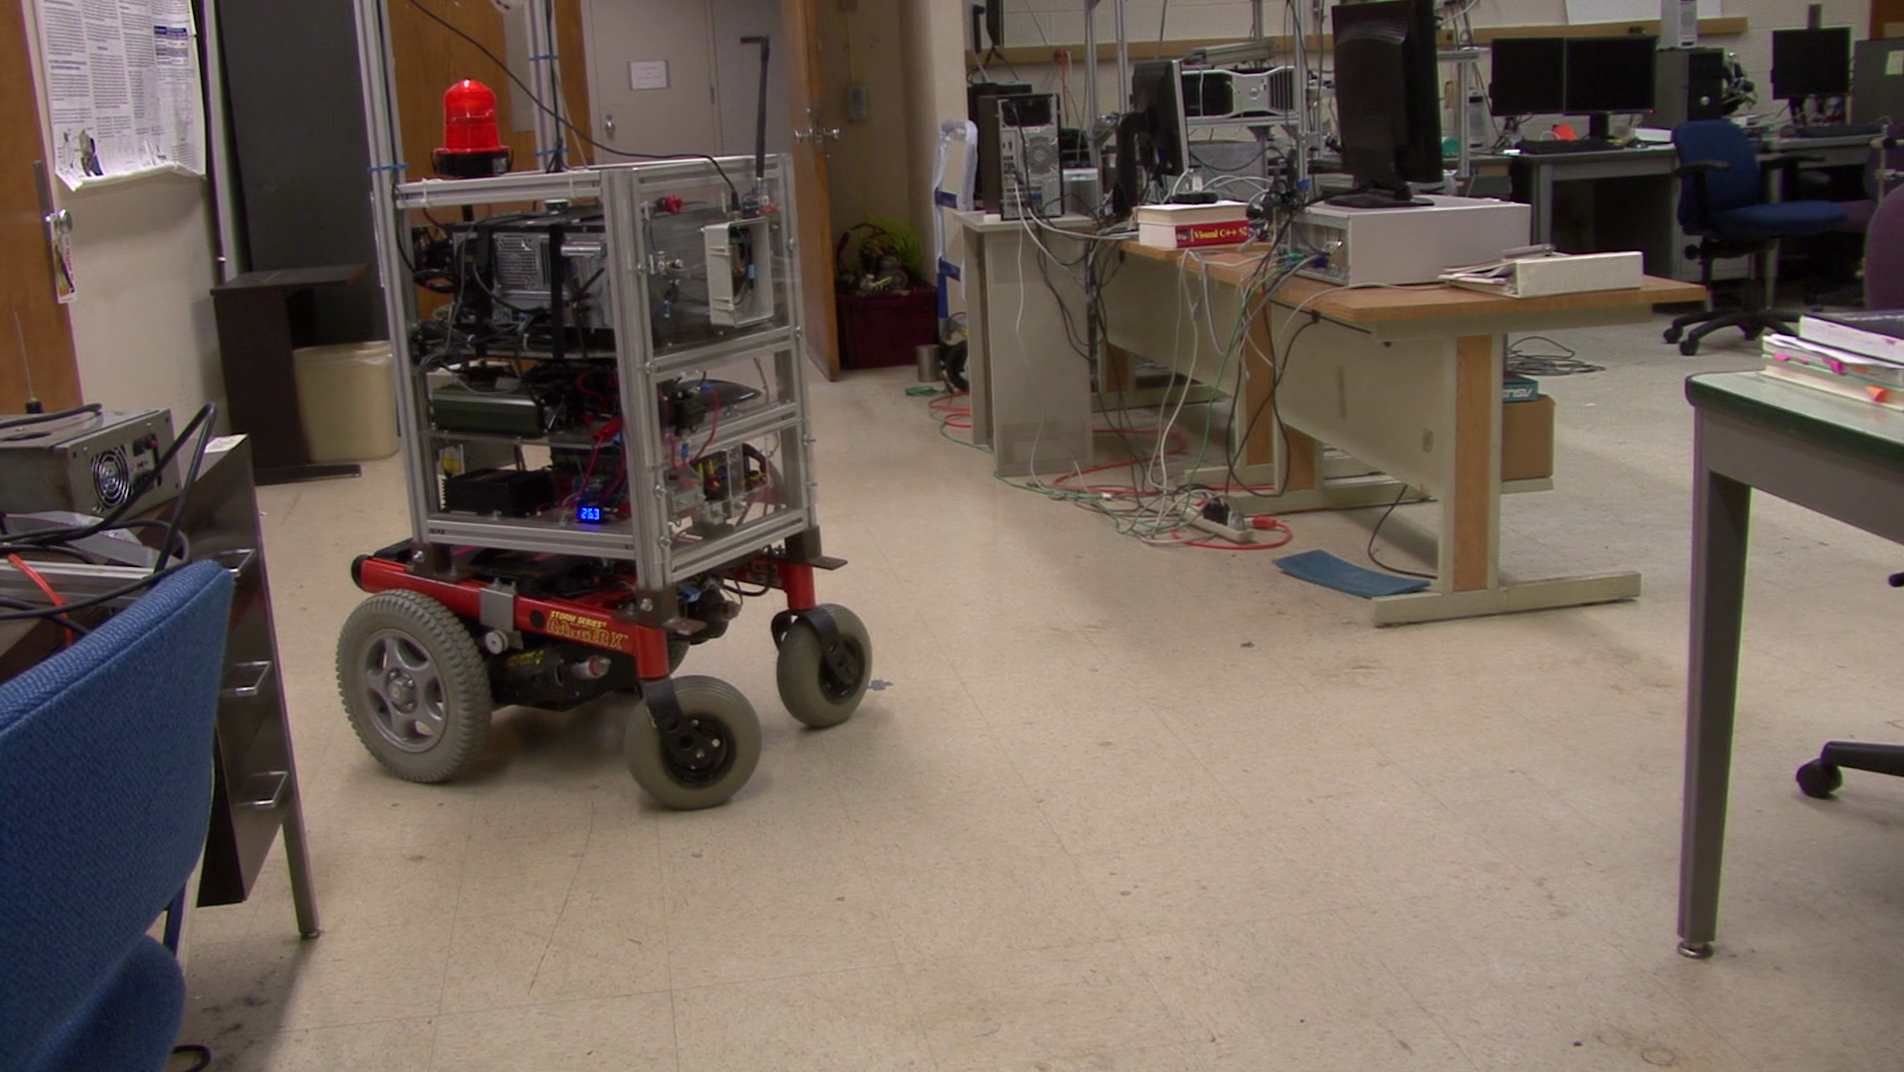
\includegraphics[width=0.49\textwidth]{images/door_skill_harlie_initial_b}\label{fig:door_skill_harlie_results_initial_b}}
\\
\subfloat[Clearing Doorway]{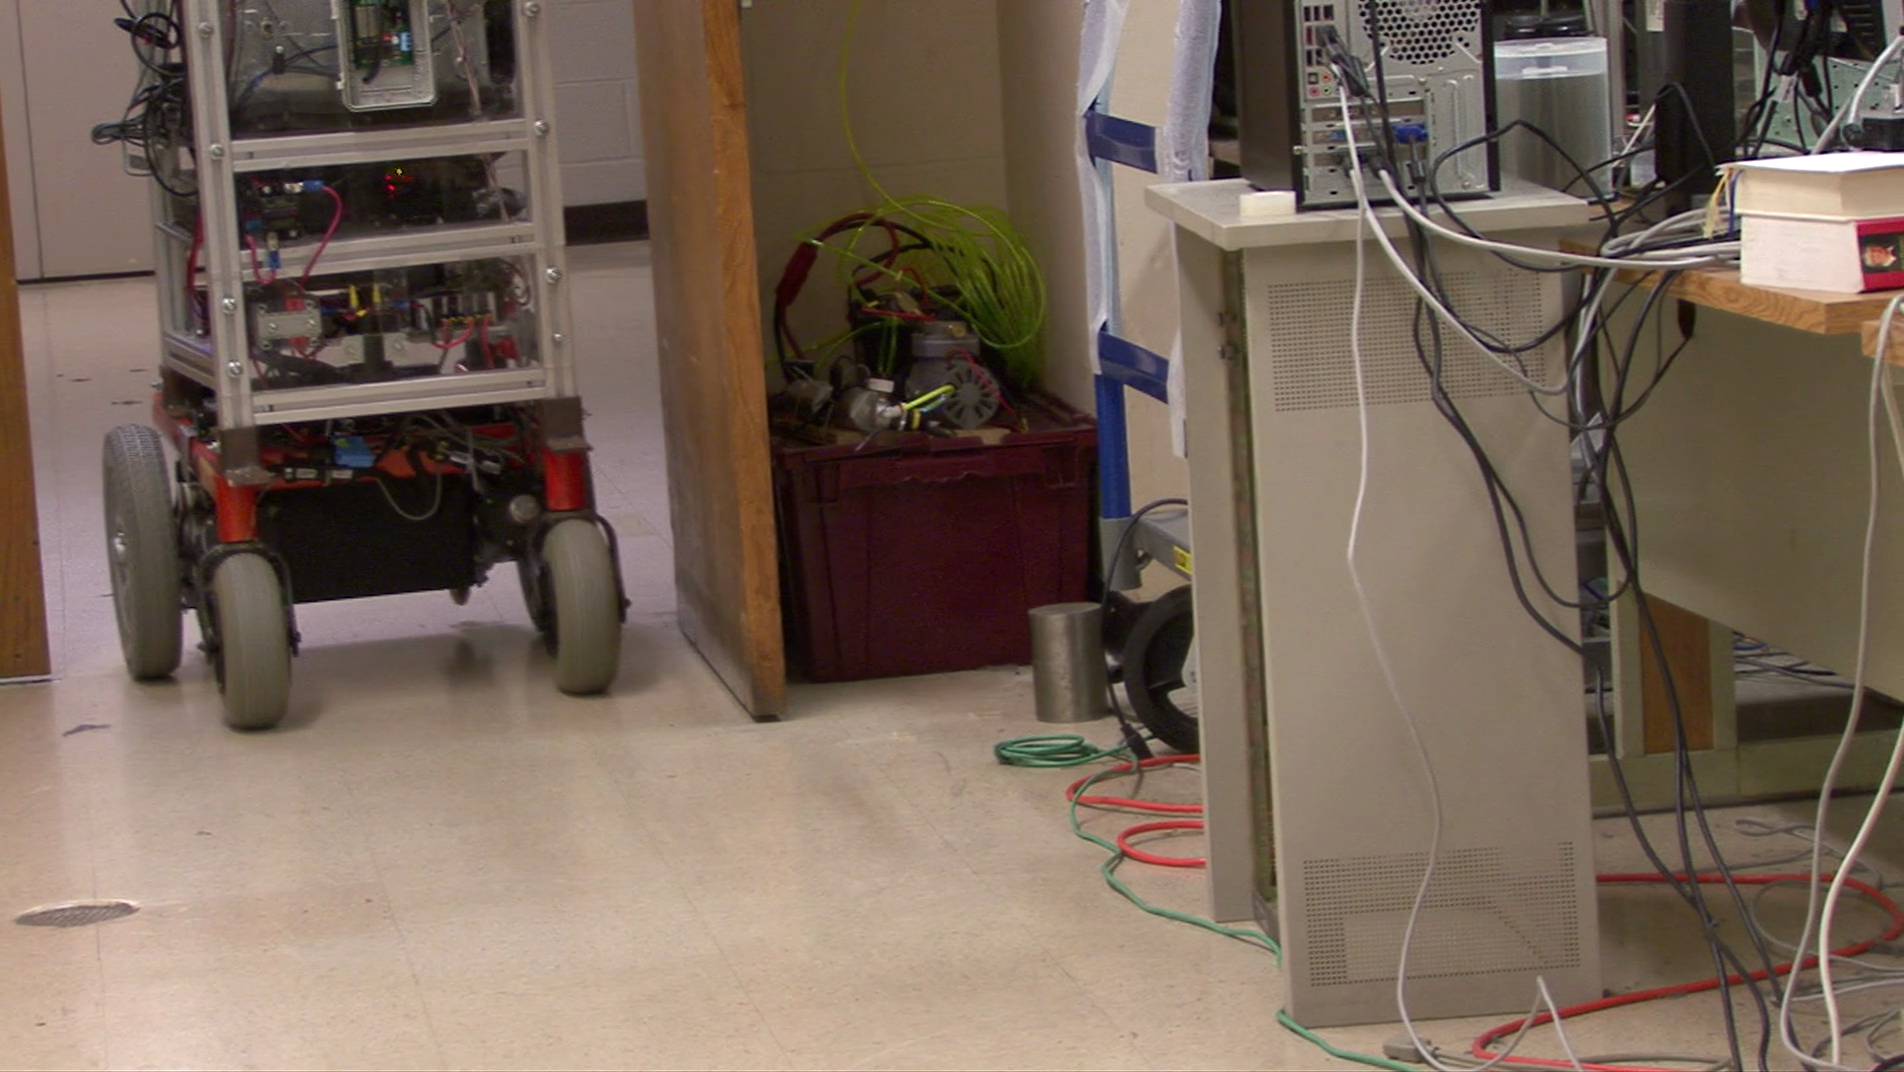
\includegraphics[width=0.75\textwidth]{images/door_skill_harlie_clearing_doorway}\label{fig:door_skill_harlie_results_clearing_doorway}}
\caption[``Door'' Test HARLIE Results]{``Door'' Test HARLIE Results. These are images captured from videos taken during the tests. The desired path runs through the middle of the door, perpendicular to the doorway.}
\label{fig:door_skill_harlie_results}
\end{figure}

\subsubsection{``Tangent'' Test}\label{subsubsec:tangent_test}

The ``tangent'' test is designed to ask: Given a set of initial conditions (lateral offset and heading error), will phase space steering converge onto the path and reach the desired end pose without overshooting? Overshooting, in this case, is defined as the robot going more than four centimeters to the other side of the desired path (this approximates a task where the robot has been commanded to pull up very closely to a wall without hitting the wall). This test involved commanding a path composed of a single straight line segment, positioned and oriented such that the line is parallel and near to a wall, while positioning the robot such that it had different lateral offsets and heading offsets to the path. These tests were conducted both in the Gazebo simulation environment described in \autoref{subsec:simulation_setup} and a subset of those results were tested on HARLIE to verify that the simulation results transfered to the physical robot. Simulation results are shown in \autoref{fig:tangent_skill_sim_results}, where a tangential distance of more than five meters means that no overshoot occurred before the end of the desired path.

\begin{figure}
\centering
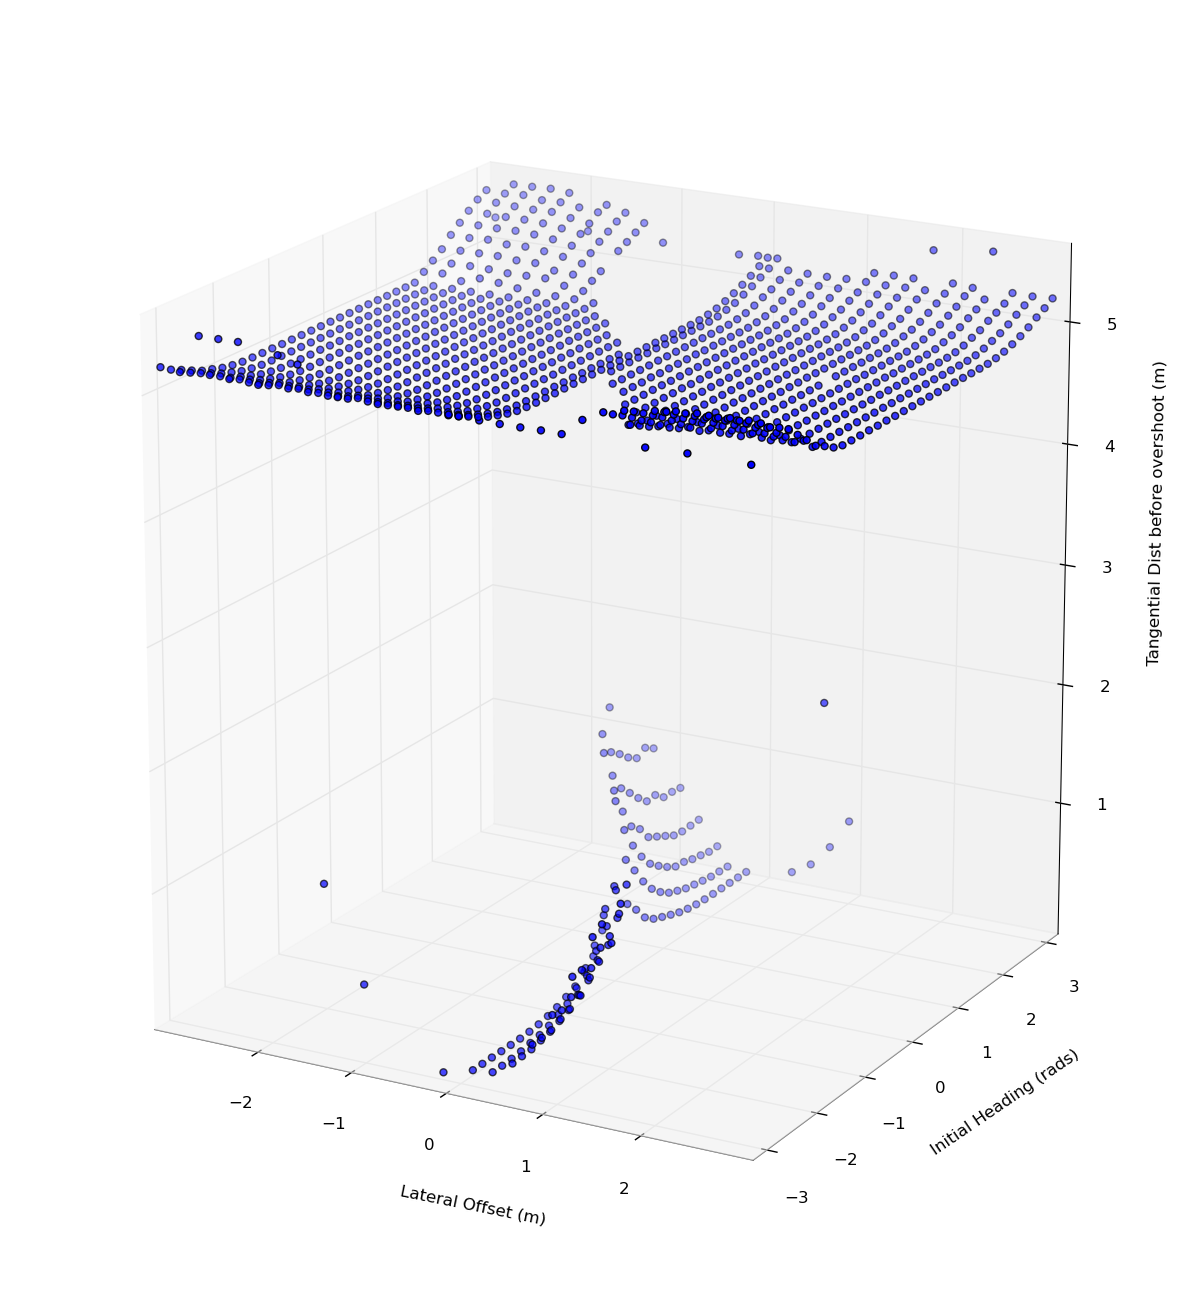
\includegraphics[width=0.95\textwidth]{images/acceptable_overshoot_scatter}
\caption[``Tangent'' Test Simulation Results]{``Tangent'' Test Simulation Results. The X-axis is the Initial Heading Error (rads), the Y-axis is the Initial Lateral Offset Error (m) and the Z-axis is the Tangential Distance before Overshoot (m).}
\label{fig:tangent_skill_sim_results}
\end{figure}

\autoref{fig:tangent_skill_sim_results} shows a number of useful results. The first is that, just as with the ``door'' test results, the performance is symmetric about the XZ-plane. It also indicates that the likelihood of overshooting is greatly influenced by the the lateral offset from the path -- the less lateral offset the robot starts with, the more likely it is to overshoot the desired path while converging.

This experiment also yielded information on the set of initial conditions that are acceptable for how far the robot can go without overshooting a given path. An example of such a path is a smart wheelchair pulling up next to a handicap door assist button. Similarly to the ``door'' test results, these results can be used to determine whether a path planner must replan a path from the robot's current position to the origin of the desired path or if the desired path can be commanded directly with no replanning. For example, the data collected in simulation implies that, given a lateral offset of one meter and an initial heading error of ninety degrees, overshooting will occur; in that situation, it would not be safe to directly command the desired path if the desired path required no overshooting. A number of runs were conducted with HARLIE to validate these results; these tests with the physical system confirmed the simulation results. See \autoref{fig:tangent_skill_harlie_results} for some examples of HARLIE while conducting these tests. One particular initial condition (see \autoref{fig:tangent_skill_harlie_results_initial}) as well as HARLIE successfully stopping parallel to a card reader that would unlock the door (see \autoref{fig:tangent_skill_harlie_results_approaching_reader}).

\begin{figure}
\centering
\subfloat[Initial Condition]{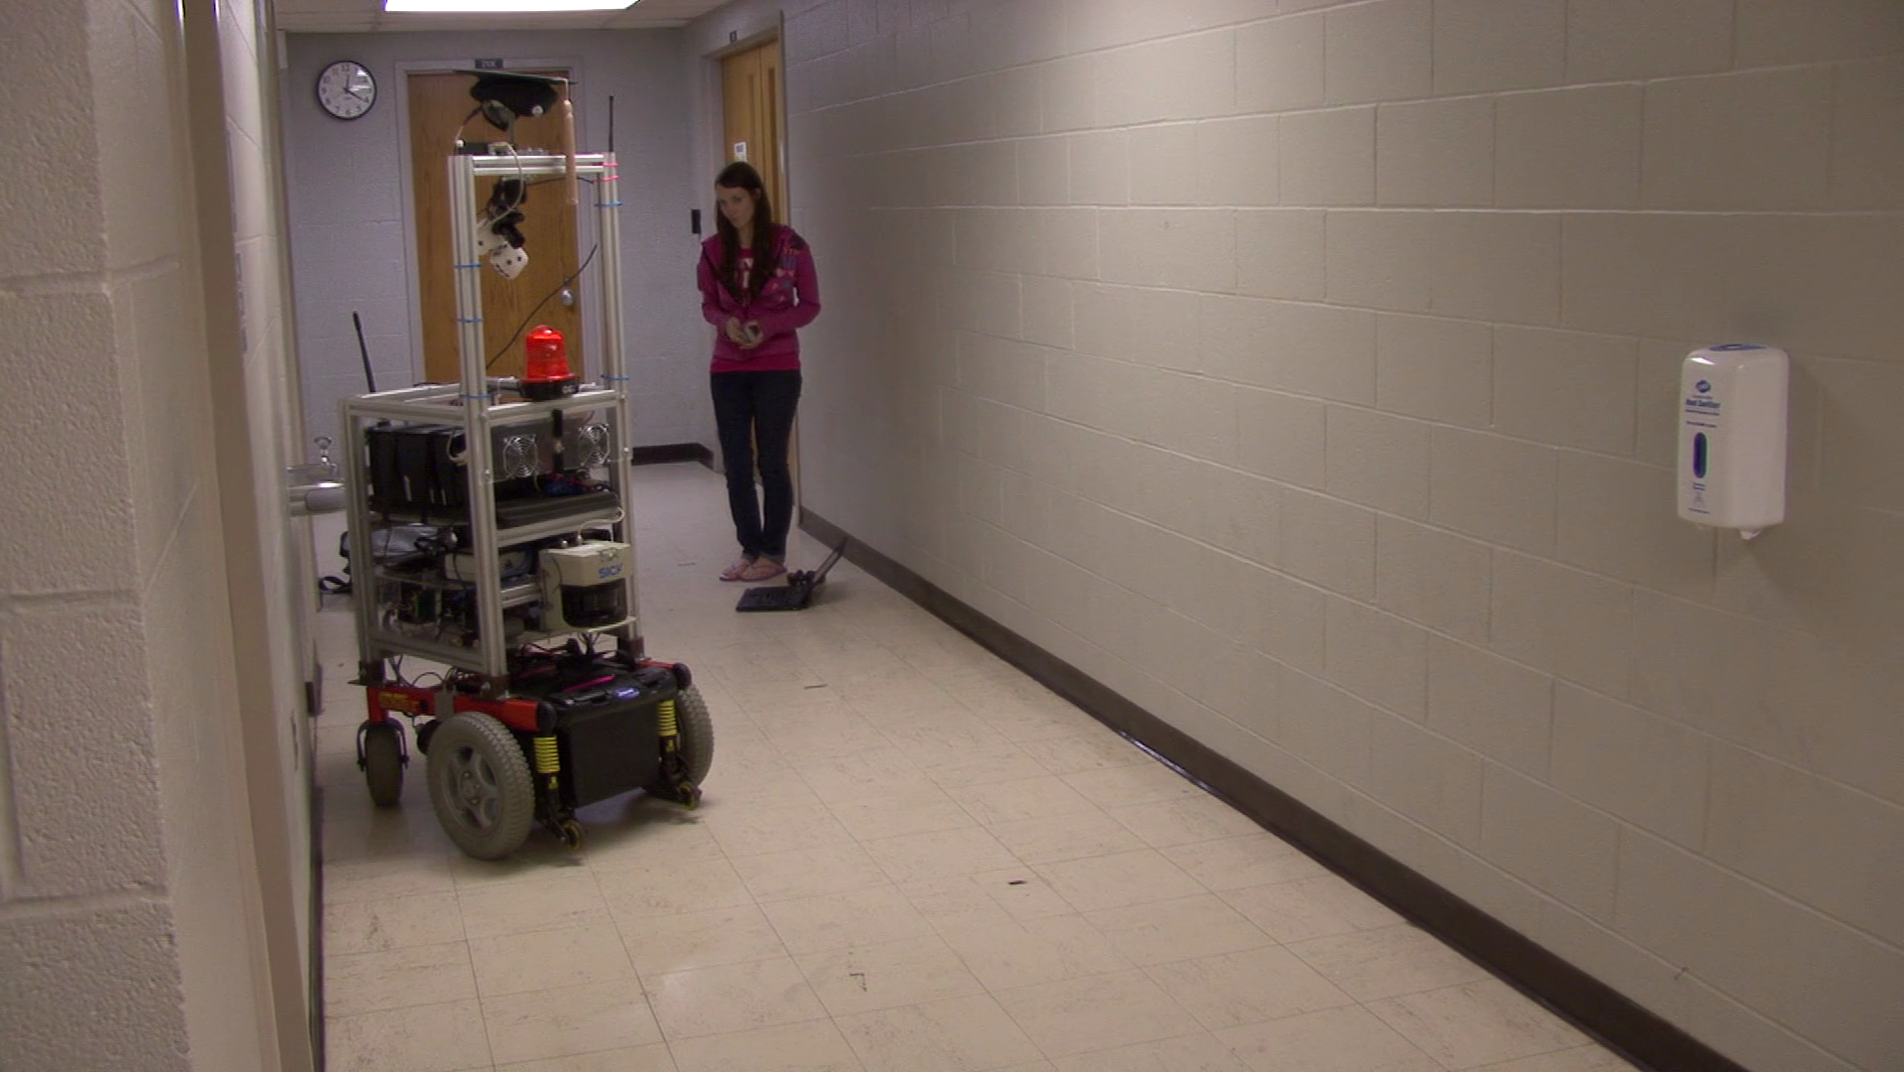
\includegraphics[width=0.75\textwidth]{images/tangent_skill_harlie_initial}\label{fig:tangent_skill_harlie_results_initial}}
\\
\subfloat[Stopping Parallel to Card Reader]{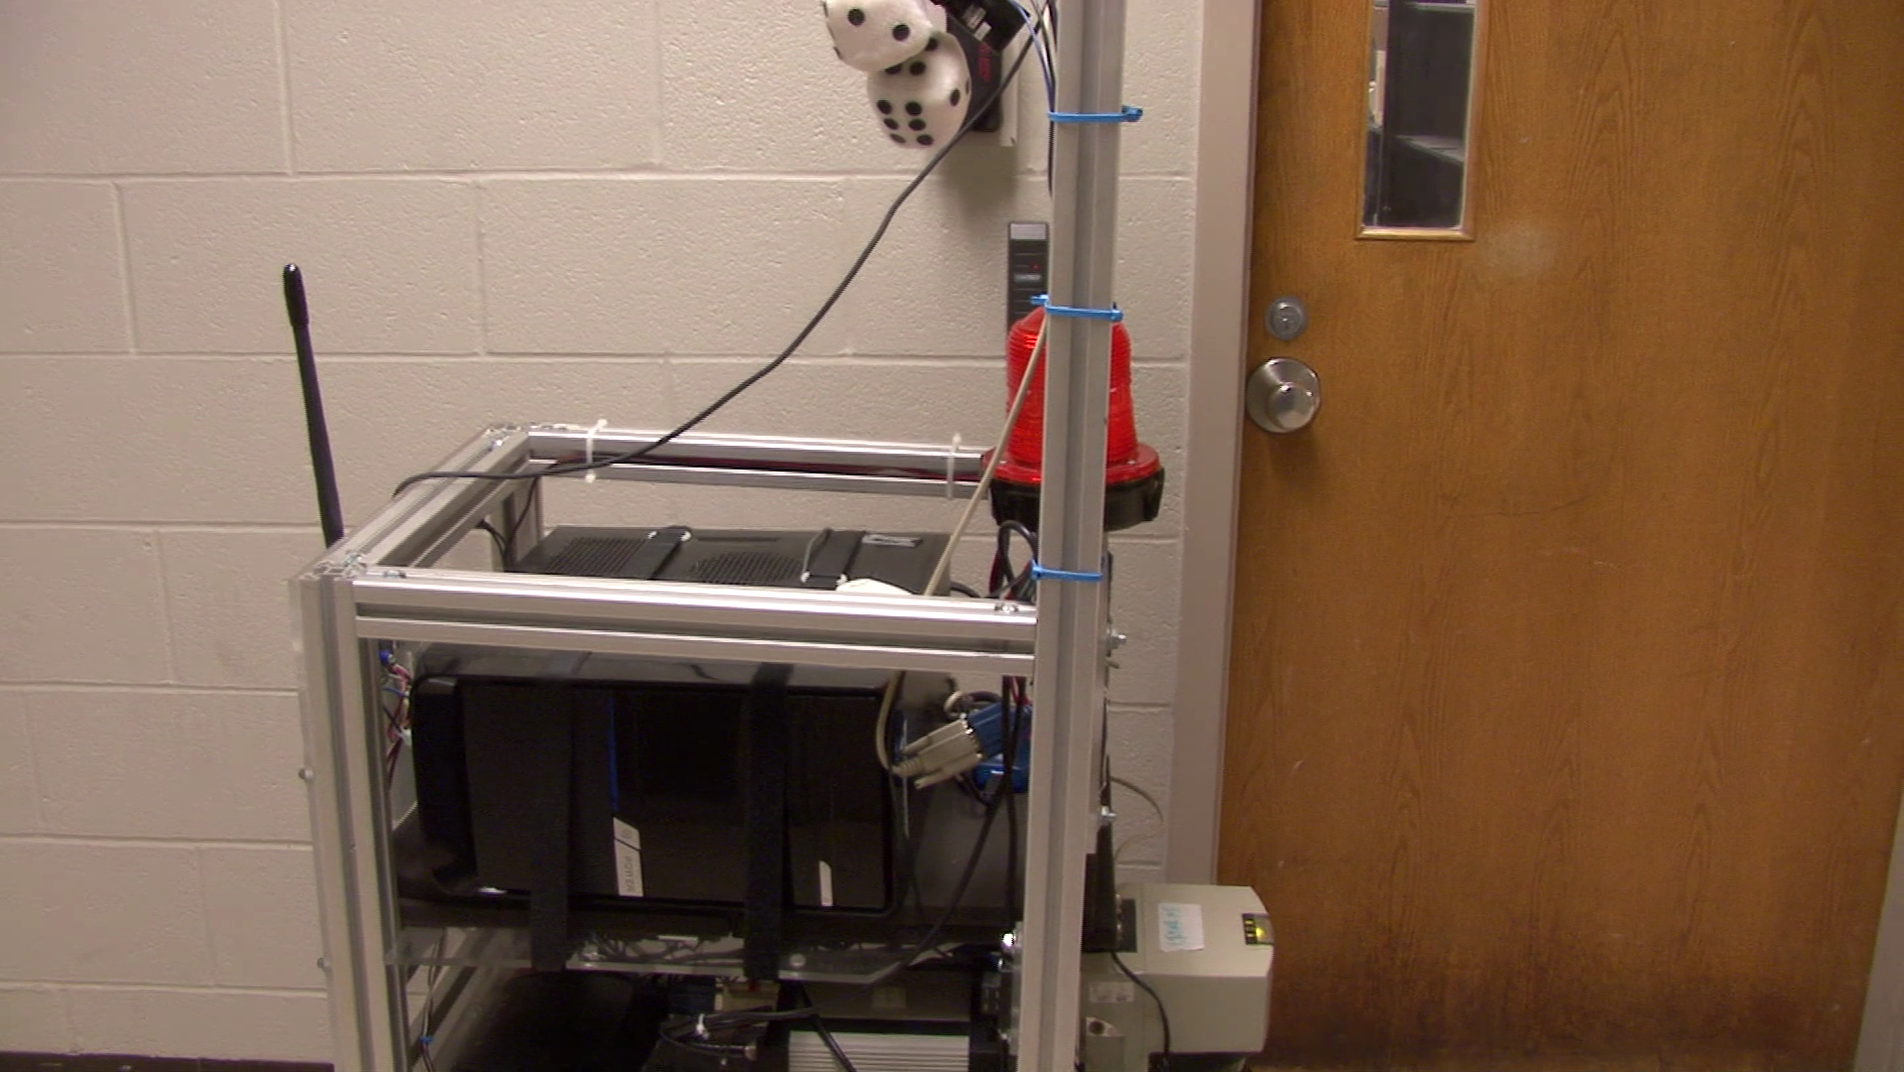
\includegraphics[width=0.75\textwidth]{images/tangent_skill_harlie_approaching_reader}\label{fig:tangent_skill_harlie_results_approaching_reader}}
\caption[``Tangent'' Test HARLIE Results]{``Tangent'' Test HARLIE Results. These are images captured from videos taken during the tests. The desired path runs parallel to the wall.}
\label{fig:tangent_skill_harlie_results}
\end{figure}

\subsection{Splicing Tests}\label{subsec:splicing_tests}

Experiments were also conducted to validate the splicing method described in \autoref{sec:path_planning}. In this test, HARLIE was given a path where the first segment was a long straight line. This segment was then blocked with an orange construction barrel in order to force the planner to splice in a path around it. An example from one of these tests is in \autoref{fig:splicing_test_results}. \autoref{fig:splicing_test_results_pre_splice} shows HARLIE while waiting for the planner to splice a path around the barrel; the barrel is the semicircle in the laser scan and obstacle map immediately in front and to the right of HARLIE. \autoref{fig:splicing_test_results_after_splice} shows HARLIE after fifteen seconds of waiting for the barrel to move; the planner spliced in a sequence of segments as described in \autoref{sec:path_planning} and HARLIE began executing the newly spliced path segments. \autoref{fig:splicing_test_results_post_splice_segment} shows HARLIE after finishing the spliced segments and resuming the original path segment after successfully avoiding the barrel.

While these experiments validated that the splicing method described in \autoref{sec:path_planning} worked in some cases, they also confirmed some of the limitations of that splicing method. For example, in the first experiment the one meter radius of the spliced in semicircle was insufficient. After HARLIE started executing the spliced in path, the path was still going to result in a collision with the barrel. In order for HARLIE to complete the path in that experiment, the barrel had to be moved away from the path. This result led to increasing the radius of the spliced in semicircle to two meters for the results shown in \autoref{fig:splicing_test_results}.

\begin{figure}
\centering
\subfloat[HARLIE Stopped, Waiting for Obstacle to Move]{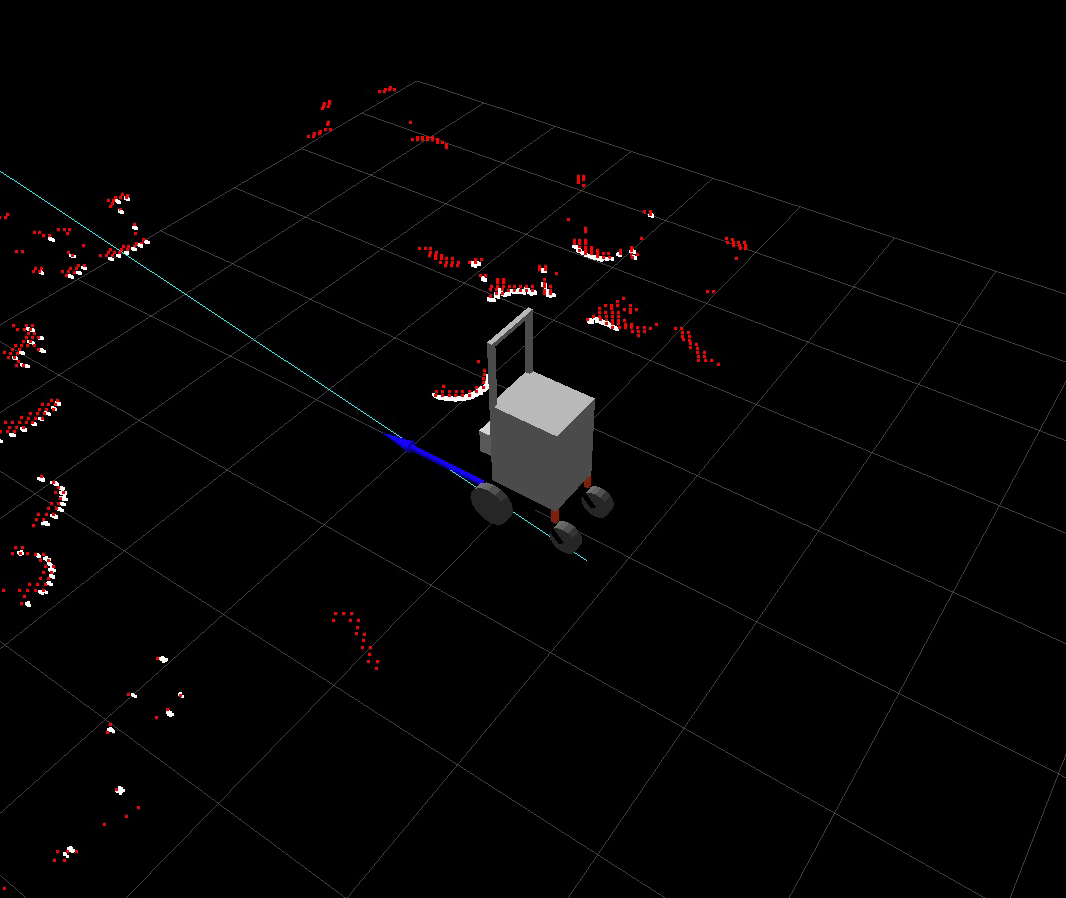
\includegraphics[width=0.70\textwidth]{images/splicing_test_pre_splice}\label{fig:splicing_test_results_pre_splice}}
\\
\subfloat[HARLIE Post-Splicing, On Spliced Arc]{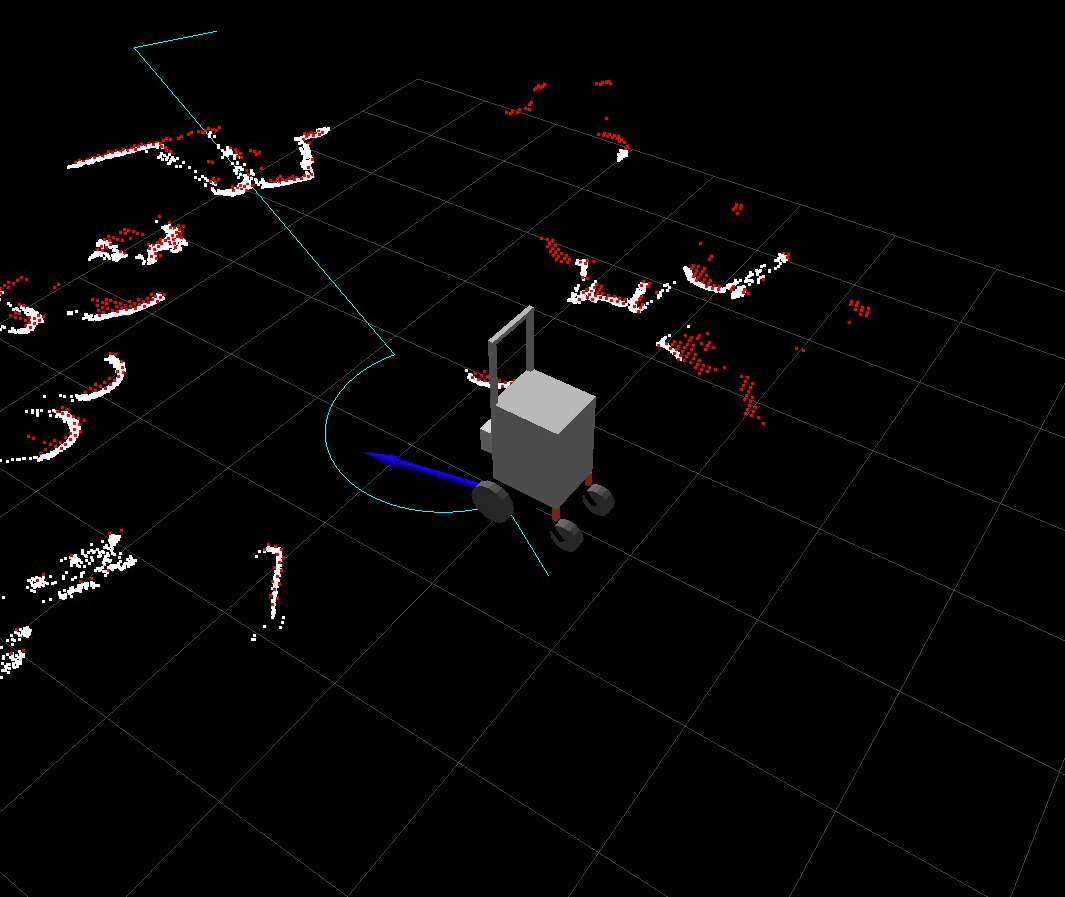
\includegraphics[width=0.70\textwidth]{images/splicing_test_after_splice}\label{fig:splicing_test_results_after_splice}}
\caption[Splicing Test Results Figures (a) and (b)]{Splicing Test Results  Figures (a) and (b).}
\end{figure}

\begin{figure}
\centering
\ContinuedFloat
\subfloat[HARLIE Post-Splicing, Resuming Original Line Segment]{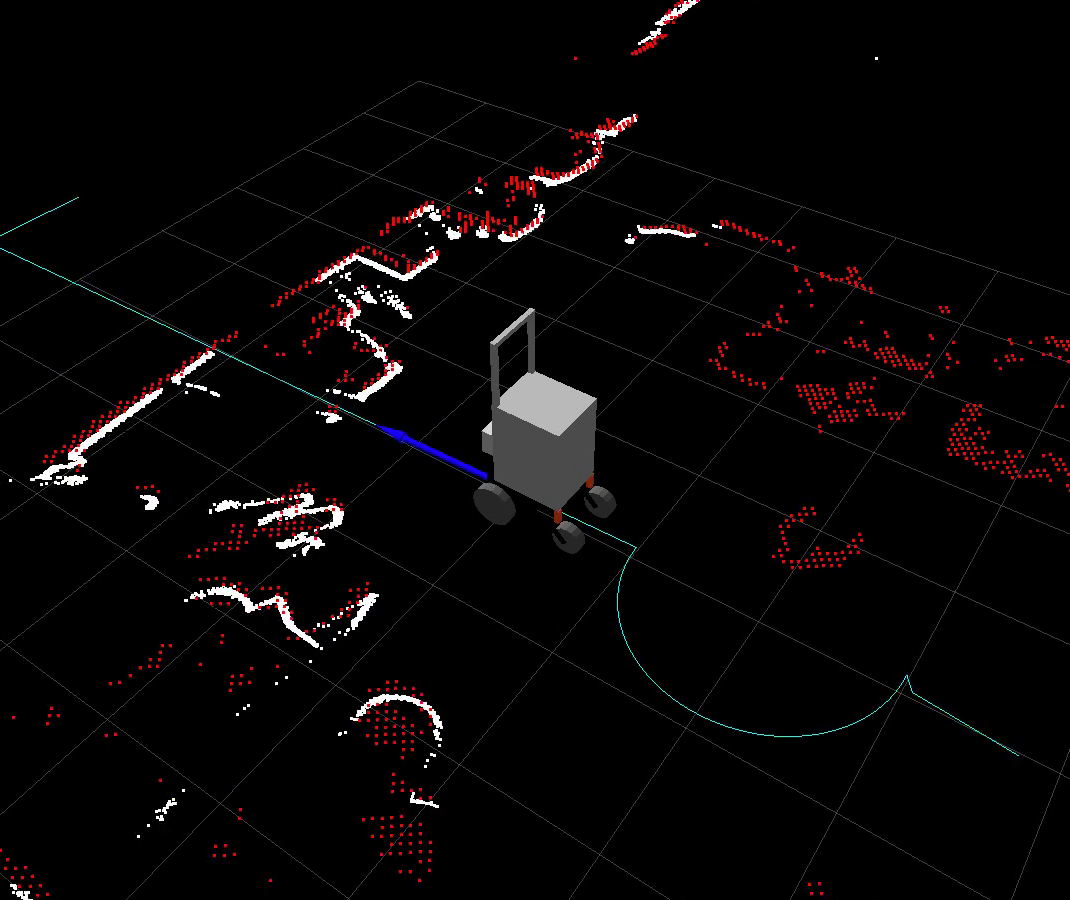
\includegraphics[width=0.70\textwidth]{images/splicing_test_post_splice_segment}\label{fig:splicing_test_results_post_splice_segment}}
\caption[Splicing Test Results Figure (c)]{Splicing Test Results Figure (c). These are images captured from videos of the GUI taken during the tests. Teal line is the desired path, blue arrow is the current desired state, red is the obstacle data from ``costmap3d'', white is the current laser scan and the set of polygons is a model of HARLIE.}
\label{fig:splicing_test_results}
\end{figure}

\begin{comment}

* Navigation on hallway and figure 8
* Joystick control results on same for comparison

* Skills
	* Door Skill
	* Tangent Skill

* Splicing

\end{comment}